\section{Marco teórico}

\subsection*{Raspberry Pi 3 B+}
\begin{itemize}
	\item Funciona con un sistema operativo basado en la arquitectura ARM.
	\item Módulo Wi-Fi de banda dual de 2,4 y 5 GHz.
	\item 40 pines Entrada/Salida de Propósito General (GPIO)
	\item Salidas de 3.3 y 5 V, buses I²C, SPI
\end{itemize}

\begin{figure}[htb]
	\centering
	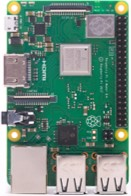
\includegraphics[scale=0.5]{raspberrypi.jpg}
	\caption{Raspberry Pi 3 B+}
\end{figure}

\subsection*{Qt}
\begin{itemize}
	\item Optimizada para aplicaciones con interfaces gráficas en sistemas embebidos.
	\item Soporte para C++
	\item Utiliza el lenguaje declarativo QML para programar la interfaz
\end{itemize}

\begin{figure}[htb]
	\centering
	
\includegraphics[scale=0.5]{qt.jpg}
	\caption{Logotipo de Qt Framework}
\end{figure}

\subsection*{Bus I2C}
\begin{itemize}
	\item Bus serial de comunicación de tipo maestro-esclavo.
	\item Línea serial de datos bidireccional (SDA)  y línea serial de reloj (SCL).
	\item Espacio de direcciones, cada dirección identifica a un dispositivo conectado al bus.
\end{itemize}

\begin{figure}[htb]
	\centering
	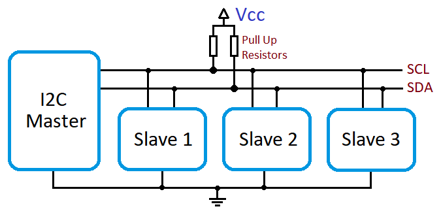
\includegraphics[scale=0.5]{i2c.png}
	\caption{Diagrama del bus I2C}
\end{figure}

\subsection*{Bus SPI}
\begin{itemize}
	\item Bus serial de comunicación de tipo maestro-esclavo.
	\item Líneas de entrada al esclavo (MOSI) y salida al esclavo (MISO), línea de reloj (SCLK).
	\item Línea de selección del chip (SS).
\end{itemize}

\begin{figure}[htb]
	\centering
	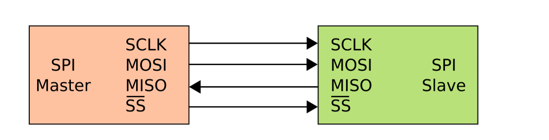
\includegraphics[scale=0.5]{spi.png}
	\caption{Diagrama del bus SPI}
\end{figure}

\subsection*{MPU-6050}
\begin{itemize}
	\item Giroscopio de vibración de Coriolis y acelerómetro de 3 ejes.
	\item Procesador de movimiento digital (DMP) que mide la orientación del sensor en tres ejes.
	\item Buffer FIFO interno.
	\item Filtro paso bajo.
	\item Comunicación por medio del bus I²C de hasta 400 KHz.
	\item Pin AD0 para cambiar la dirección en el bus. Solo puede tomar las direcciones 104 y 105.
\end{itemize}

\begin{figure}[htb]
	\centering
	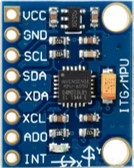
\includegraphics[scale=0.5]{mpu6050.jpg}
	\caption{Sensor inercial MPU6050}
\end{figure}

\subsection*{MPU-9250}
\begin{itemize}
	\item Giroscopio de vibración de Coriolis y acelerómetro de 3 ejes.
	\item Procesador de movimiento digital (DMP) que mide la orientación del sensor en tres ejes.
	\item Buffer FIFO interno.
	\item Filtro paso bajo.
	\item Comunicación por medio del bus SPI de hasta 10 MHz.
\end{itemize}

\begin{figure}[htb]
	\centering
	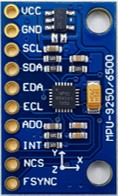
\includegraphics[scale=0.4]{mpu9250.jpg}
	\caption{Sensor inercial MPU9250}
\end{figure}

%\subsection*{Sensor flexible capacitivo}
%\begin{itemize}
%	\item Mide el ángulo de torsión al que se somete el sensor en una dirección.
%	\item El valor medido es una resistencia variable
%\end{itemize}

%\begin{figure}[htb]
%	\centering
%	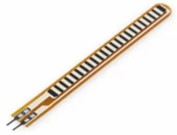
\includegraphics[scale=0.6]{flexsensor.jpg}
%	\caption{Sensor flexible capacitivo}
%\end{figure}

%\subsection*{Convertidor analógico-digital MCP3004}
%\begin{itemize}
%	\item Voltaje de referencia de 2,7 V a 5,5 V
%\end{itemize}

%\begin{figure}[htb]
%	\centering
%	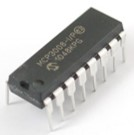
\includegraphics[scale=0.6]{mcp3004.jpg}
%	\caption{Convertidor A/D MCP3004}
%\end{figure}

\subsection*{Microservomotor posicional}
\begin{itemize}
	\item Ángulo de entrada de 0° a 180°
	\item Utiliza señales de modulación de ancho de pulso (PWM)
	\item Movimiento bidireccional
\end{itemize}

\begin{figure}[htb]
	\centering
	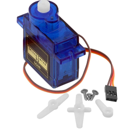
\includegraphics[scale=0.6]{servomotor.png}
	\caption{Microservomotor posicional}
\end{figure}